% Copyright (c) 2017 Alexander Bluhm <bluhm@openbsd.org>
%
% Permission to use, copy, modify, and distribute this software for any
% purpose with or without fee is hereby granted, provided that the above
% copyright notice and this permission notice appear in all copies.
%
% THE SOFTWARE IS PROVIDED "AS IS" AND THE AUTHOR DISCLAIMS ALL WARRANTIES
% WITH REGARD TO THIS SOFTWARE INCLUDING ALL IMPLIED WARRANTIES OF
% MERCHANTABILITY AND FITNESS. IN NO EVENT SHALL THE AUTHOR BE LIABLE FOR
% ANY SPECIAL, DIRECT, INDIRECT, OR CONSEQUENTIAL DAMAGES OR ANY DAMAGES
% WHATSOEVER RESULTING FROM LOSS OF USE, DATA OR PROFITS, WHETHER IN AN
% ACTION OF CONTRACT, NEGLIGENCE OR OTHER TORTIOUS ACTION, ARISING OUT OF
% OR IN CONNECTION WITH THE USE OR PERFORMANCE OF THIS SOFTWARE.

\documentclass[14pt]{beamer}
\usetheme{Frankfurt}
\usepackage{tikz}
\usetikzlibrary{shapes.geometric}
\author{Alexander Bluhm}
\title{Never Loose a Syslog Message}
\institute{\url{bluhm@openbsd.org}}
\date{September 24, 2017}

\begin{document}

\begin{frame}
\titlepage
\end{frame}

\section{Motivation}

\begin{frame}{Agenda}
\setcounter{tocdepth}{1}
\tableofcontents
\end{frame}

\subsection{Why reliable logging?}
\begin{frame}{Why reliable logging?}
\begin{itemize}
    \item system analysis
    \item attacker tries to prevent log
    \item required by common criteria
\end{itemize}
\end{frame}

\subsection{What can go wrong?}
\begin{frame}{What can go wrong?}
\begin{itemize}
    \item UDP for remote logs
    \item UNIX datagram for local logs
    \item file descriptors
    \item chroot environment
    \item timestamps and time zones
\end{itemize}
\end{frame}

\section{Starting Position}

\subsection{Traditional Message Flow}
\begin{frame}{Traditional Message Flow}
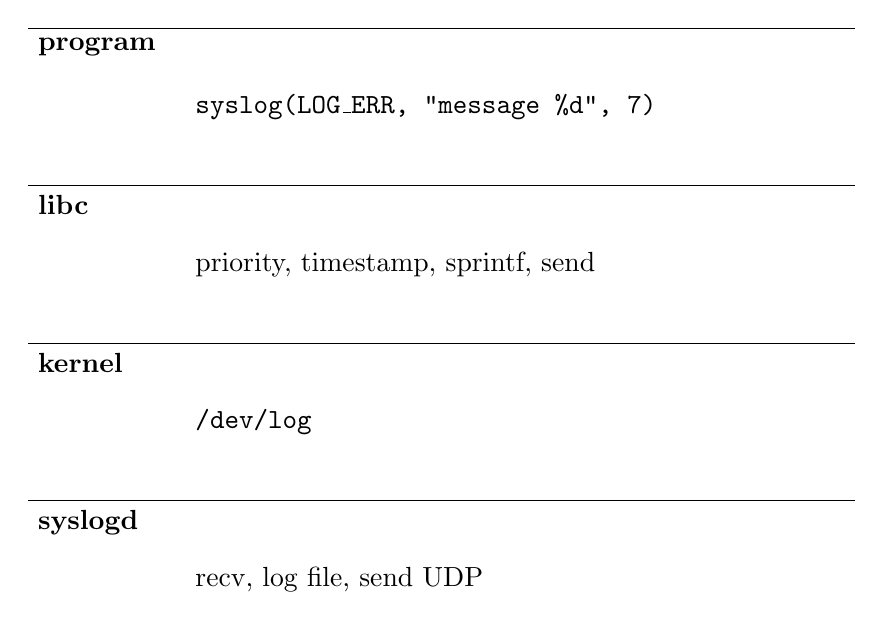
\begin{tikzpicture}
\draw
    ++(0,-2) node[anchor=north west]{\textbf{program}} -- +(10.5,0)
    +(2,-1) node[anchor=west]{\texttt{syslog(LOG\_ERR, "message \%d", 7)}}
    ++(0,-2) node[anchor=north west]{\textbf{libc}}    -- +(10.5,0)
    +(2,-1) node[anchor=west]{priority, timestamp, sprintf, send}
    ++(0,-2) node[anchor=north west]{\textbf{kernel}}  -- +(10.5,0)
    +(2,-1) node[anchor=west]{\texttt{/dev/log}}
    ++(0,-2) node[anchor=north west]{\textbf{syslogd}} -- +(10.5,0)
    +(2,-1) node[anchor=west]{recv, log file, send UDP};
\end{tikzpicture}
\end{frame}

\subsection{Priority, Facility, Level, Severity, Options}
\begin{frame}{Priority, Facility, Level, Severity, Options}
    \texttt{openlog("ftpd", LOG\_PID|LOG\_CONS, LOG\_FTP)}\\
    \texttt{syslog(LOG\_INFO, "\%s logged in", user)}

    \vspace{.5cm}
    \texttt{\#define LOG\_FTP  (11<<3) /* ftp daemon */}\\
    \texttt{\#define LOG\_INFO 6       /* informational */ }

    \vspace{.5cm}
    \texttt{<94>Sep 24 09:35:00 ftpd[4711]:\ bluhm logged in}
\end{frame}

\section{Local Improvements}

\subsection{/dev/log}
\begin{frame}{/dev/log}
Problems with \texttt{/dev/log} UNIX socket
\begin{itemize}
    \item needs file descriptor
    \item use \texttt{LOG\_NDELAY}
    \item reconnect after \texttt{SIGHUP} syslogd
    \item needs UNIX socket in chroot
    \item needs \texttt{pledge("unix")}
    \item LOG\_CONS is even worse
\end{itemize}
\end{frame}

\subsection{sendsyslog}
\begin{frame}{sendsyslog}
    New system call sendsyslog(2)

    \vspace{.5cm}
    \texttt{int \\
    sendsyslog(const void *msg, size\_t len, int flags)}

    \vspace{.5cm}
    \texttt{sendsyslog("<94>Sep 24 09:36:23 ftpd[4711]:\
	bluhm logged in", 47, LOG\_CONS)}
\end{frame}

\subsection{Using sendsyslog}
\begin{frame}{Using sendsyslog}
    Syslogd does
\begin{itemize}
    \item create socketpair
    \item register one end with \texttt{ioctl(LIOCSFD)}
    \item receive form other end
\end{itemize}
    \vspace{.5cm}
    Kernel does
\begin{itemize}
    \item send to syslogd's socketpair
    \item write to console if necessary
    \item ktrace if activated
    \item count errors
\end{itemize}
\end{frame}

\subsection{Error Handling}
\begin{frame}{Error Handling}
    \texttt{void \\
	syslog(int prio, const char *msg, ...)}
\begin{itemize}
    \item libc cannot return error
    \item program cannot log error
\end{itemize}
    \vspace{.5cm}
    Kernel sendsyslog can do it
\begin{itemize}
    \item count failures when sending to syslogd
    \item write message to syslog when it works again
\end{itemize}
    \vspace{.5cm}
    \texttt{sendsyslog:\ dropped 2 messages, error 57}
\end{frame}

\subsection{Libc Timestamp}
\begin{frame}{Libc Timestamp}
    Timestamp from syslog(3)
\begin{itemize}
    \item needs \texttt{/etc/localtime} in every chroot
    \item no year
    \item no time zone
    \item no indication of daylight saving time
    \item insufficient precision
    \item does not work for kernel messages
\end{itemize}
    \vspace{.5cm}
    \texttt{Sep 24 09:37:42}
\end{frame}

\subsection{Syslogd Timestamp}
\begin{frame}{Syslogd Timestamp}
    Timestamp added by syslogd
\begin{itemize}
    \item timestamp is optional in received message
    \item syslogd adds it if missing
    \item libc does not generate it
    \item syslogd -Z generates ISO format in UTC
    \item use millisecond precision
\end{itemize}
    \vspace{.5cm}
    \texttt{2017-09-24T07:38:59.333}
\end{frame}

\subsection{Logging without Libc}
\begin{frame}{Logging without Libc}
    System call sendsyslog allows logging
\begin{itemize}
    \item from signal handler
    \item at memcpy overlap
    \item from stack protector handler
    \item from ld.so dynamic linker
\end{itemize}
\end{frame}

\subsection{dmesg Overflow}
\begin{frame}{dmesg Overflow}
    Detect dmesg overflow in log file
\begin{itemize}
    \item ring buffer with kernel logs
    \item syslogd reads from \texttt{/dev/klog}
    \item messages may overwrite
    \item special kernel message at gap
\end{itemize}
    \vspace{.5cm}
    \texttt{<4>klog:\ dropped 1243 bytes, message buffer full}
\end{frame}

\section{Remote Logging}

\subsection{Possibilities}
\begin{frame}{Possibilities}
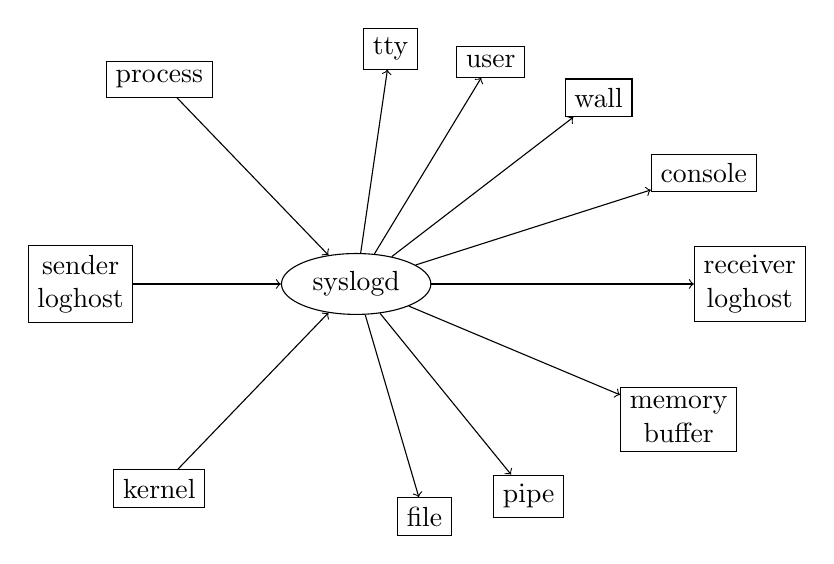
\begin{tikzpicture}
\node [draw,ellipse]      (syslogd)  at (   0, 0) {syslogd};
\node [draw,align=center] (sender)   at (-3.5, 0) {sender\\ loghost};
\node [draw,align=center] (receiver) at (   5, 0) {receiver\\ loghost};

\node [draw]              (tty)      at
    (xyz polar cs:angle=85,x radius=5,y radius=3) {tty};
\node [draw]              (user)     at
    (xyz polar cs:angle=70,x radius=5,y radius=3) {user};
\node [draw]              (wall)     at
    (xyz polar cs:angle=52,x radius=5,y radius=3) {wall};
\node [draw]              (console)  at
    (xyz polar cs:angle=28,x radius=5,y radius=3) {console};
\node [draw,align=center] (pipe)     at
    (xyz polar cs:angle=-35,x radius=5,y radius=3) {memory\\ buffer};
\node [draw]              (file)     at
    (xyz polar cs:angle=-64,x radius=5,y radius=3) {pipe};
\node [draw]              (memory)   at
    (xyz polar cs:angle=-80,x radius=5,y radius=3) {file};

\node [draw]              (process)  at
    (xyz polar cs:angle=120,x radius=5,y radius=3) {process};
\node [draw]              (kernel)   at
    (xyz polar cs:angle=240,x radius=5,y radius=3) {kernel};
\draw [->] (node cs:name=sender) -- (node cs:name=syslogd);
\draw [->] (node cs:name=process) -- (node cs:name=syslogd);
\draw [->] (node cs:name=kernel) -- (node cs:name=syslogd);
\draw [->] (node cs:name=syslogd) -- (node cs:name=receiver);
\draw [->] (node cs:name=syslogd) -- (node cs:name=tty);
\draw [->] (node cs:name=syslogd) -- (node cs:name=user);
\draw [->] (node cs:name=syslogd) -- (node cs:name=wall);
\draw [->] (node cs:name=syslogd) -- (node cs:name=console);
\draw [->] (node cs:name=syslogd) -- (node cs:name=memory);
\draw [->] (node cs:name=syslogd) -- (node cs:name=pipe);
\draw [->] (node cs:name=syslogd) -- (node cs:name=file);
\end{tikzpicture}
\end{frame}

\subsection{Local Methods}
\begin{frame}{Local Methods}
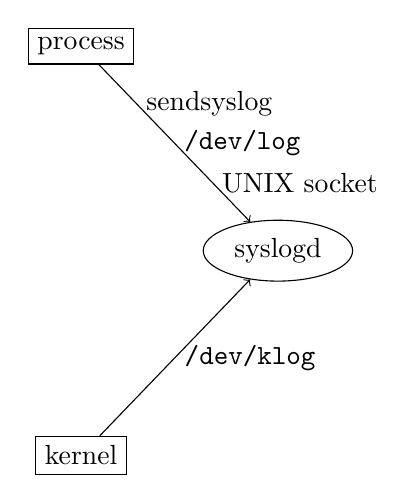
\begin{tikzpicture}
\node [draw,ellipse]      (syslogd)  at ( 0, 0) {syslogd};
\node [draw]              (process)  at
    (xyz polar cs:angle=120,x radius=5,y radius=3) {process};
\node [draw]              (kernel)   at
    (xyz polar cs:angle=240,x radius=5,y radius=3) {kernel};

\draw [->] (node cs:name=process) --
    node[near start,anchor=west] {sendsyslog}
    node[anchor=west]            {\texttt{/dev/log}}
    node[near end,anchor=west]   {UNIX socket}
    (node cs:name=syslogd);
\draw [->] (node cs:name=kernel) --
    node[anchor=west] {\texttt{/dev/klog}}
    (node cs:name=syslogd);
\end{tikzpicture}
\end{frame}

\subsection{Remote Methods}
\begin{frame}{Remote Methods}
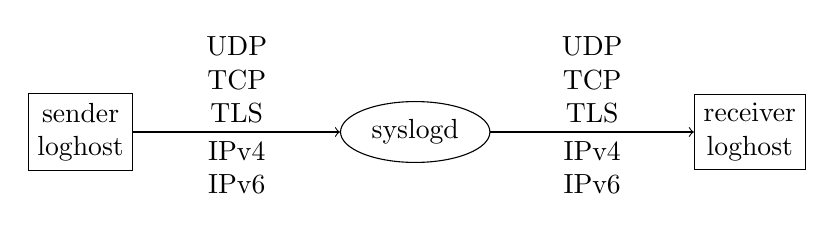
\begin{tikzpicture}
\node [draw,ellipse]      (syslogd)  at (    0, 0) {syslogd};
\node [draw,align=center] (sender)   at (-4.25, 0) {sender\\ loghost};
\node [draw,align=center] (receiver) at ( 4.25, 0) {receiver\\ loghost};

\draw [->] (node cs:name=sender) --
    node[align=center,anchor=south] {UDP\\ TCP\\ TLS}
    node[align=center,anchor=north] {IPv4\\ IPv6}
    (node cs:name=syslogd);
\draw [->] (node cs:name=syslogd) --
    node[align=center,anchor=south] {UDP\\ TCP\\ TLS}
    node[align=center,anchor=north] {IPv4\\ IPv6}
    (node cs:name=receiver);
\end{tikzpicture}
\end{frame}

\subsection{UDP Format}
\begin{frame}{UDP Format}
\begin{itemize}
    \item single UDP packet
    \item max 1180 bytes
\end{itemize}
    \texttt{<94>Sep 24 10:07:13 80.154.94.47 ftpd[4711]:\ bluhm logged in}
\end{frame}

\subsection{TCP Format}
\begin{frame}{TCP Format}
\begin{itemize}
    \item no propper RFC 6587
    \item new line delimiter
    \item or NUL delimiter
    \item or octet counting
\end{itemize}
    \texttt{60 <94>Sep 24 10:08:52 80.154.94.47 ftpd[4711]:\ bluhm logged in}
\end{frame}

\subsection{TLS Format}
\begin{frame}{TLS Format}
\begin{itemize}
    \item octet counting
    \item must support 2048 bytes
    \item should support 8192 bytes
    \item libevent and libtls
\end{itemize}
\end{frame}

\subsection{Provide Server Certificate}
\begin{frame}{Provide Server Certificate}
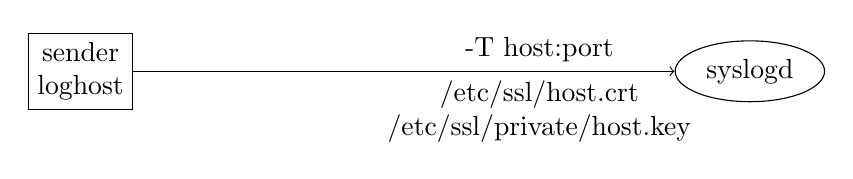
\begin{tikzpicture}
\node [draw,ellipse]      (syslogd)  at (   0, 0) {syslogd};
\node [draw,align=center] (sender)   at (-8.5, 0) {sender\\ loghost};

\draw [->] (node cs:name=sender) --
    node[near end,align=center,anchor=south]
	{-T host:port}
    node[near end,align=center,anchor=north]
	{/etc/ssl/host.crt\\ /etc/ssl/private/host.key}
    (node cs:name=syslogd);
\end{tikzpicture}
\begin{itemize}
    \item syslogd must provide server certificate
    \item sender can identify syslogd
    \item attacker cannot see messages
\end{itemize}
\end{frame}

\subsection{Validate Client Certificate}
\begin{frame}{Validate Client Certificate}
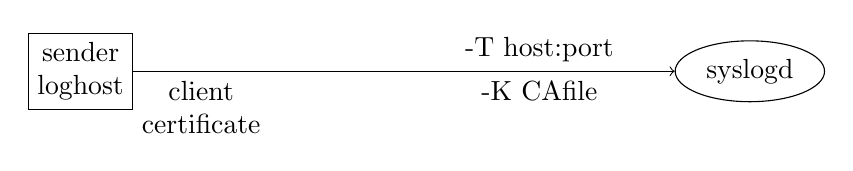
\begin{tikzpicture}
\node [draw,ellipse]      (syslogd)  at (   0, 0) {syslogd};
\node [draw,align=center] (sender)   at (-8.5, 0) {sender\\ loghost};

\draw [->] (node cs:name=sender) --
    node[near end,align=center,anchor=south]
	{-T host:port}
    node[very near start,align=center,anchor=north]
	{client\\ certificate}
    node[near end,align=center,anchor=north]
	{-K CAfile}
    (node cs:name=syslogd);
\end{tikzpicture}
\begin{itemize}
    \item sender may provide client certificate
    \item syslogd can identify sender
    \item attacker cannot inject messages
\end{itemize}
\end{frame}

\subsection{Validate Server Certificate}
\begin{frame}{Validate Server Certificate}
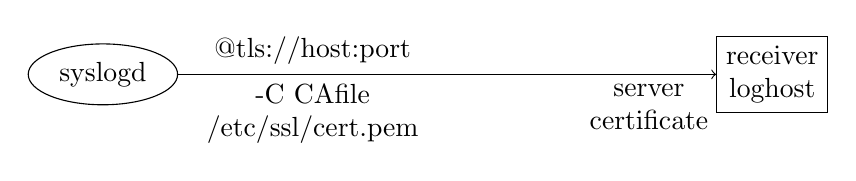
\begin{tikzpicture}
\node [draw,ellipse]      (syslogd)  at ( 0, 0) {syslogd};
\node [draw,align=center] (receiver) at (8.5, 0) {receiver\\ loghost};

\draw [->] (node cs:name=syslogd) --
    node[near start,align=center,anchor=south]
	{@tls://host:port}
    node[near start,align=center,anchor=north]
	{-C CAfile\\ /etc/ssl/cert.pem}
    node[very near end,align=center,anchor=north]
	{server\\ certificate}
    (node cs:name=receiver);
\end{tikzpicture}
\begin{itemize}
    \item syslogd must know server CA
    \item host must be in server certificate
    \item syslogd can identify receiver
    \item attacker cannot see messages
    \item turn off with -V
\end{itemize}
\end{frame}

\subsection{Provide Client Certificate}
\begin{frame}{Provide Client Certificate}
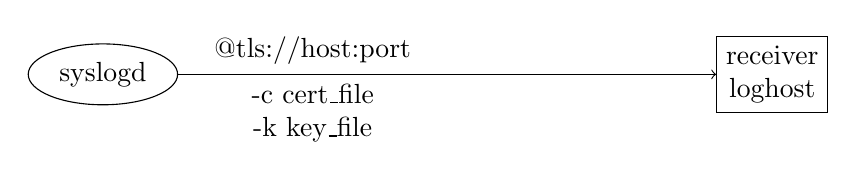
\begin{tikzpicture}
\node [draw,ellipse]      (syslogd)  at ( 0, 0) {syslogd};
\node [draw,align=center] (receiver) at (8.5, 0) {receiver\\ loghost};

\draw [->] (node cs:name=syslogd) --
    node[near start,align=center,anchor=south]
	{@tls://host:port}
    node[near start,align=center,anchor=north]
	{-c cert\_file\\ -k key\_file}
    (node cs:name=receiver);
\end{tikzpicture}
\begin{itemize}
    \item syslogd may provide client certificate
    \item sender can identify syslogd
    \item attacker cannot inject messages
\end{itemize}
\end{frame}

\subsection{TCP/TLS Errors}
\begin{frame}{TCP/TLS Errors}
\begin{itemize}
    \item debug incoming connections
    \item log connection errors
    \item count dropped messages
    \item suppress ``last message repeated''
\end{itemize}
\end{frame}

\section{Conclusion}

\subsection{OpenBSD Message Flow}
\begin{frame}{OpenBSD Message Flow}
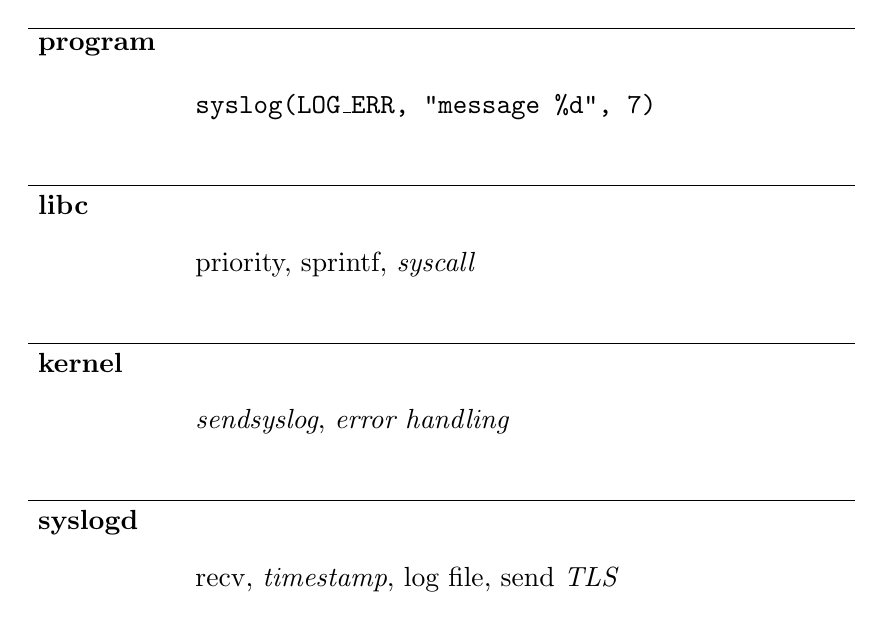
\begin{tikzpicture}
\draw
    ++(0,-2) node[anchor=north west]{\textbf{program}} -- +(10.5,0)
    +(2,-1) node[anchor=west]{\texttt{syslog(LOG\_ERR, "message \%d", 7)}}
    ++(0,-2) node[anchor=north west]{\textbf{libc}}    -- +(10.5,0)
    +(2,-1) node[anchor=west]{priority, sprintf, \textit{syscall}}
    ++(0,-2) node[anchor=north west]{\textbf{kernel}}  -- +(10.5,0)
    +(2,-1) node[anchor=west]{\textit{sendsyslog}, \textit{error handling}}
    ++(0,-2) node[anchor=north west]{\textbf{syslogd}} -- +(10.5,0)
    +(2,-1) node[anchor=west]{recv, \textit{timestamp}, log file,
	send \textit{TLS}};
\end{tikzpicture}
\end{frame}

\subsection{Run and Log Reliably}
\begin{frame}{Run and Log Reliably}
\begin{itemize}
    \item no fatal errors
    \item count dropped messages
    \item safe signal handlers
    \item libevent
    \item file descriptor exhaustion
    \item privsep with re-exec
    \item pledge child and parent
\end{itemize}
\end{frame}

\subsection{TODO}
\begin{frame}{TODO}
\begin{itemize}
    \item continue after file system full
    \item log memory buffer overflow
    \item initialization errors to file
    \item move format from RFC 3164 to 5424
\end{itemize}
\end{frame}

\subsection{Tests}
\begin{frame}{Tests}
\begin{itemize}
    \item 180 regression tests
    \item for almost everything
\end{itemize}
\end{frame}

\begin{frame}{Questions}
\begin{center}
\begin{tikzpicture}
\draw [font=\Huge] node {?};
\end{tikzpicture}
\end{center}
\end{frame}

\end{document}
